%
% $RCSfile$
%
% Copyright (c) 2005-2006. Christian Heller. All rights reserved.
%
% Permission is granted to copy, distribute and/or modify this document
% under the terms of the GNU Free Documentation License, Version 1.1 or
% any later version published by the Free Software Foundation; with no
% Invariant Sections, with no Front-Cover Texts and with no Back-Cover
% Texts. A copy of the license is included in the section entitled
% "GNU Free Documentation License".
%
% http://www.cybop.net
% - Cybernetics Oriented Programming -
%
% http://www.resmedicinae.org
% - Information in Medicine -
%
% Version: $Revision$ $Date$ $Author$
% Authors: Christian Heller <christian.heller@tuxtax.de>
%

\subsubsection{First Trial}
\label{first_trial_heading}

An early trial of a \emph{Res Medicinae} module was \emph{Record}, an
application for EHR management. It was a standard Java-based system and had a
\emph{Graphical User Interface} (GUI). Its classical architecture made use of
many software patterns and was shared into the parts \emph{Domain Model},
\emph{Graphical View} and \emph{Controller}, as proposed by the equally named
pattern, abbreviated \emph{MVC}.

Later prototypes extended that architecture by applying the CYBOP concept of
\emph{Composition}. In a first step, the \emph{Hierarchical MVC} (HMVC) pattern
was used to replace the MVC pattern, resulting in nested \emph{Controllers} and
\emph{Views}. Afterwards, the principle of \emph{Hierarchy} was applied in
general, also to \emph{Domain Models} and to as many other parts as possible.

Classes as known from \emph{Object Oriented Programming} (OOP) do not represent
dynamically extensible containers but have a static structure with a fixed
number of attributes. In other words, the \emph{Hierarchy} as concept is not
inherent in OOP types. Yet abstract models as humans build them in their minds
are always based on hierarchies (section \ref{reflexions_on_concepts_heading}).
A programming language which does not consider this, does not allow users to
make full use of their modelling potential.

To eliminate this flaw and implement a hierarchical structure in the Java
prototype, a top-most super class named \emph{cybop.Model} had to be introduced.
It represented a container that had the capability to reference itself -- in
other words a \emph{Tree Structure}. As such, it offered \emph{set}, \emph{get}
and \emph{remove} methods for its elements. Since these access methods were
inherited, sub classes did not have to implement their own (for each attribute)
anymore, which saved hundreds of lines of source code.

\begin{figure}[ht]
    \begin{center}
        \includegraphics[scale=0.2]{vector/topological.eps}
        \caption{Topological Documentation}
        \label{topological_figure}
    \end{center}
\end{figure}

One of these advanced modules, to give an example, was responsible for clinical
documentation \cite{hellerbohl}, which it supported graphically, in form of
\emph{Topological Documentation} (figure \ref{topological_figure}). And, of
course, it could also manage and store patient data, in XML files.
